\subsection{Result Comparison}
\hspace{12pt} Taking a look at the magnitude plots (Figure \ref{fig:mag_comp}), we can see slight differences between them, the Ngspice graph has a strange shape which is due to the bandpass filter (high-pass and low-pass stages) and the complex impedances inside de OP-AMP, while the Octave graph looks exactly like a bandpass filter we intended.

\begin{figure}[h!]
	\centering
	\subfigure[]{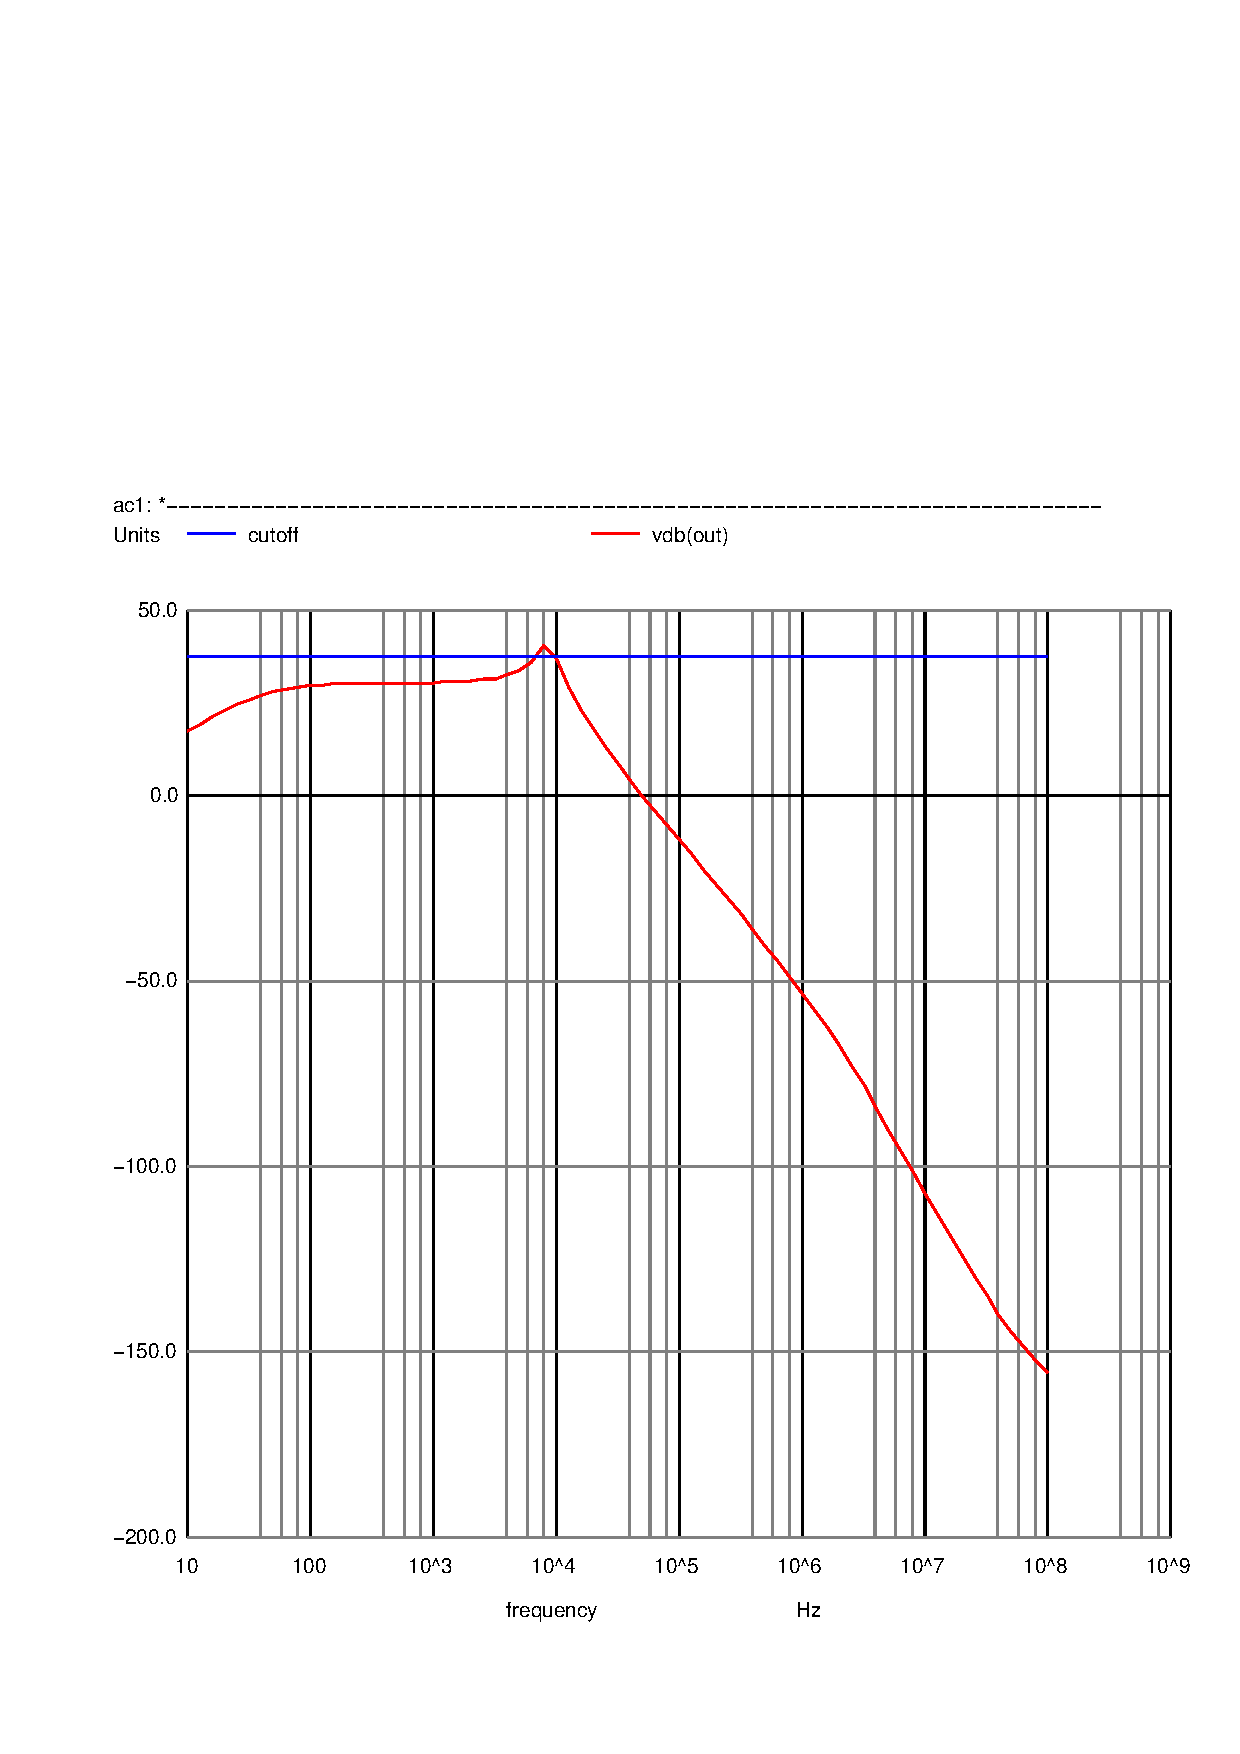
\includegraphics[width=0.3\textwidth, trim={0, 2cm, 0, 8cm}, clip]{vout_mag.pdf}}
	\subfigure[]{\includegraphics[width=0.4\textwidth, trim={0, 6cm, 0, 6cm}, clip]{gain_mag.pdf}}
	\caption{(a) Ngspice and (b) Octave magnitude plots of the frequency response output}
	\label{fig:mag_comp}
\end{figure}

\begin{figure}[h]
	\centering
	\begin{minipage}[t]{.4\textwidth}
		\centering
		\small
		\begin{tabular}{|c|c|}
		\hline
		\input{out_tab.tex}
		\normalsize
		\end{tabular}
	\end{minipage}
	\medskip
	\begin{minipage}{.4\textwidth}
		\centering
       	\input{results.tex}
	\end{minipage}
	\label{fig:op_comp}
	\caption{Results(a) Ngspice (b) Octave script}
\end{figure}

As we can see, both the results for the simulation and the theoretical analysis are very similar, in order to better see this agreement we can look at the relative error between the results:

\begin{figure}[h]
	\centering
	\begin{tabular}{|c|c|}
		\hline
		Quantity & Relative Error (\%) \\ \hline
		Lower Cutoff Frequency & -2.45321 \\ \hline
		Central Frequency & -7.62450 \\ \hline
		Upper Cutoff Frequency Frequency & -12.52166 \\ \hline
		Input Impedance & -0.496051, 21.38860\\ \hline
		Output Impedance & 0, 0\\ \hline
		Gain & 6.833636 \\ \hline
	\end{tabular}
\end{figure}

These relative errors are small in some cases (Lower cutoff freq, central freq, output impedance and gain), however, there are some differences which we can explain due to the difference between the theoretical model and the real OP-AMP component. 

\subsection{The Theoretical OP-AMP Model}
\hspace{12pt} Finally, we will take a look at the theoretical model used back in section \ref{sec:theory}, it is possible to see that, due to its simplicity, it would be very difficult to accurately represent the effect of the OP-AMP, the main difference we experienced is related to the frequency response: given that the theoretical model only includes 2 resistors and a voltage controled voltage source, it cannot model the frequency effects the real component represents (which contains 2 capacitors), this results in the difference in shape we can see in the bode plots.

\begin{figure}[h]
 	\centering
	\includegraphics[width=.5\textwidth, trim={0 2cm 0 5cm}, clip]{OP_AMP.pdf}
	\vspace{-20pt}
	\caption{OP-AMP amplifier incremental model}
	\label{fig:OP-AMP}
\end{figure}

